\section{IMPLEMENTATION}  \label{sec:implementation}
\begin{figure}%[htb]
  \centering
    \subfigure[AUV positioning - global frame of reference.] {\label{fig:auv-positioning}
	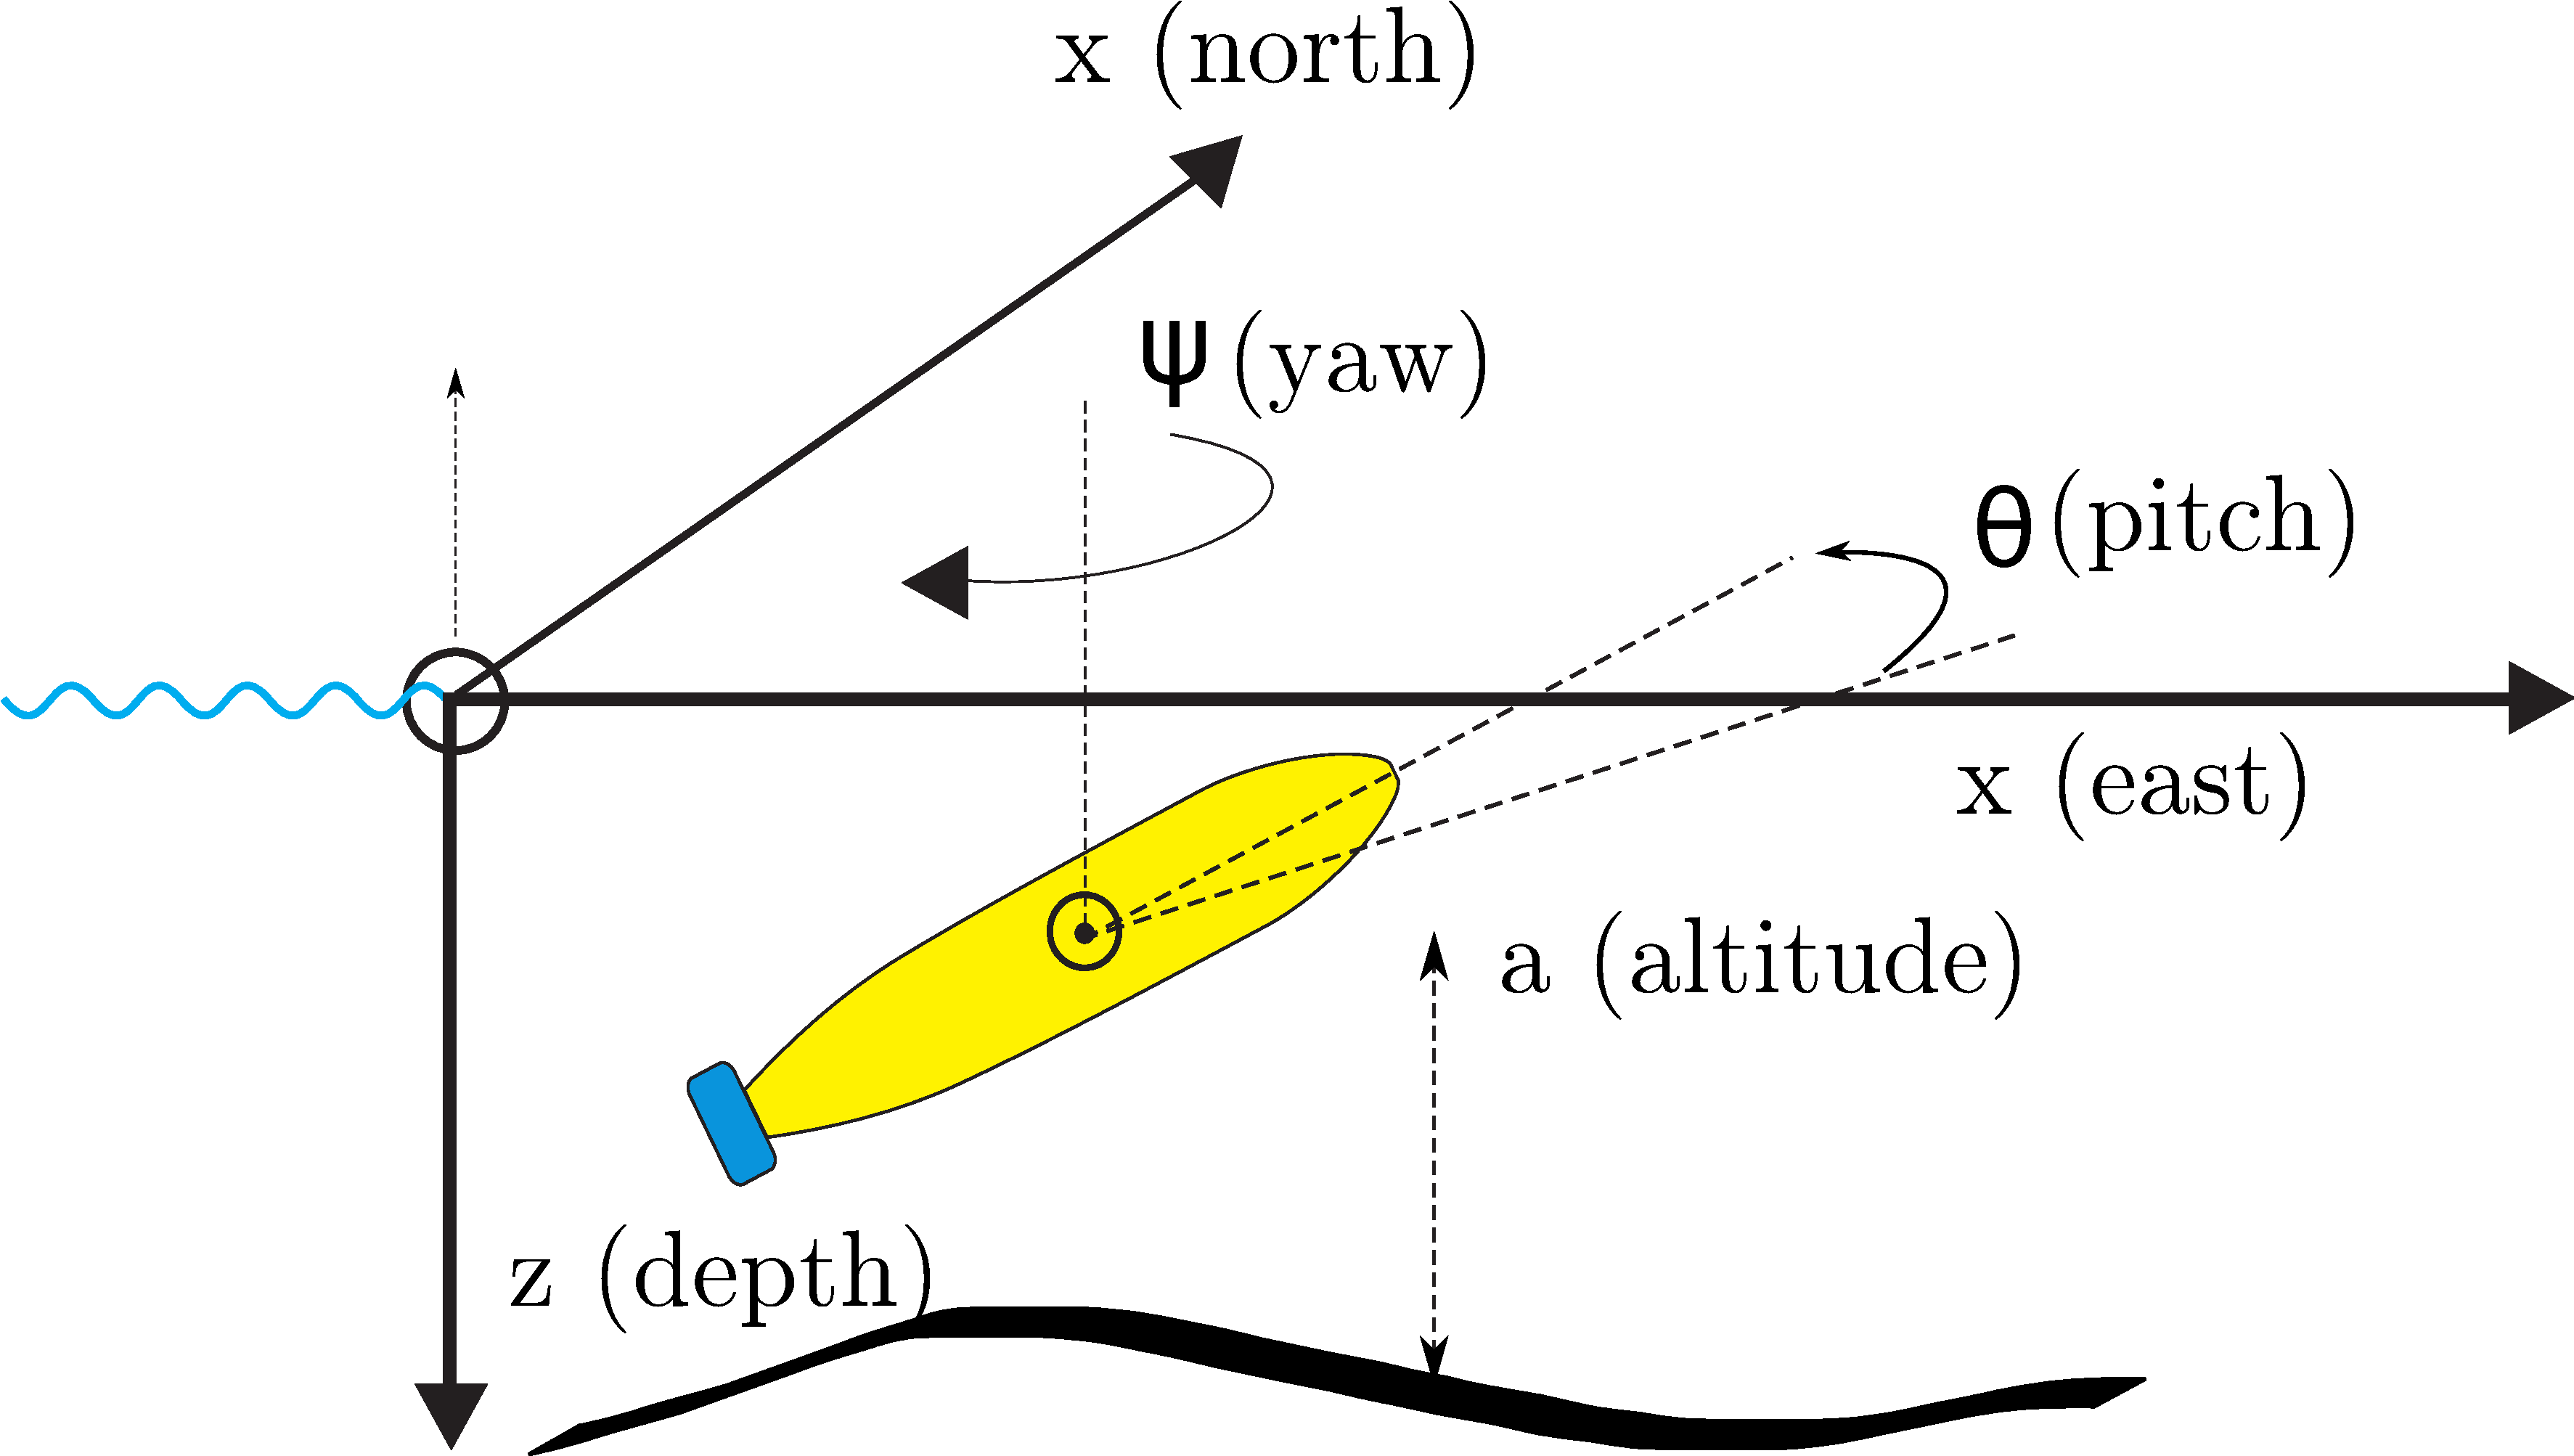
\includegraphics[width=0.8\linewidth]{auv-model.pdf}} \\
    \subfigure[AUV body frame - local coordinate system with movement directions.] {\label{fig:auv-axes}
    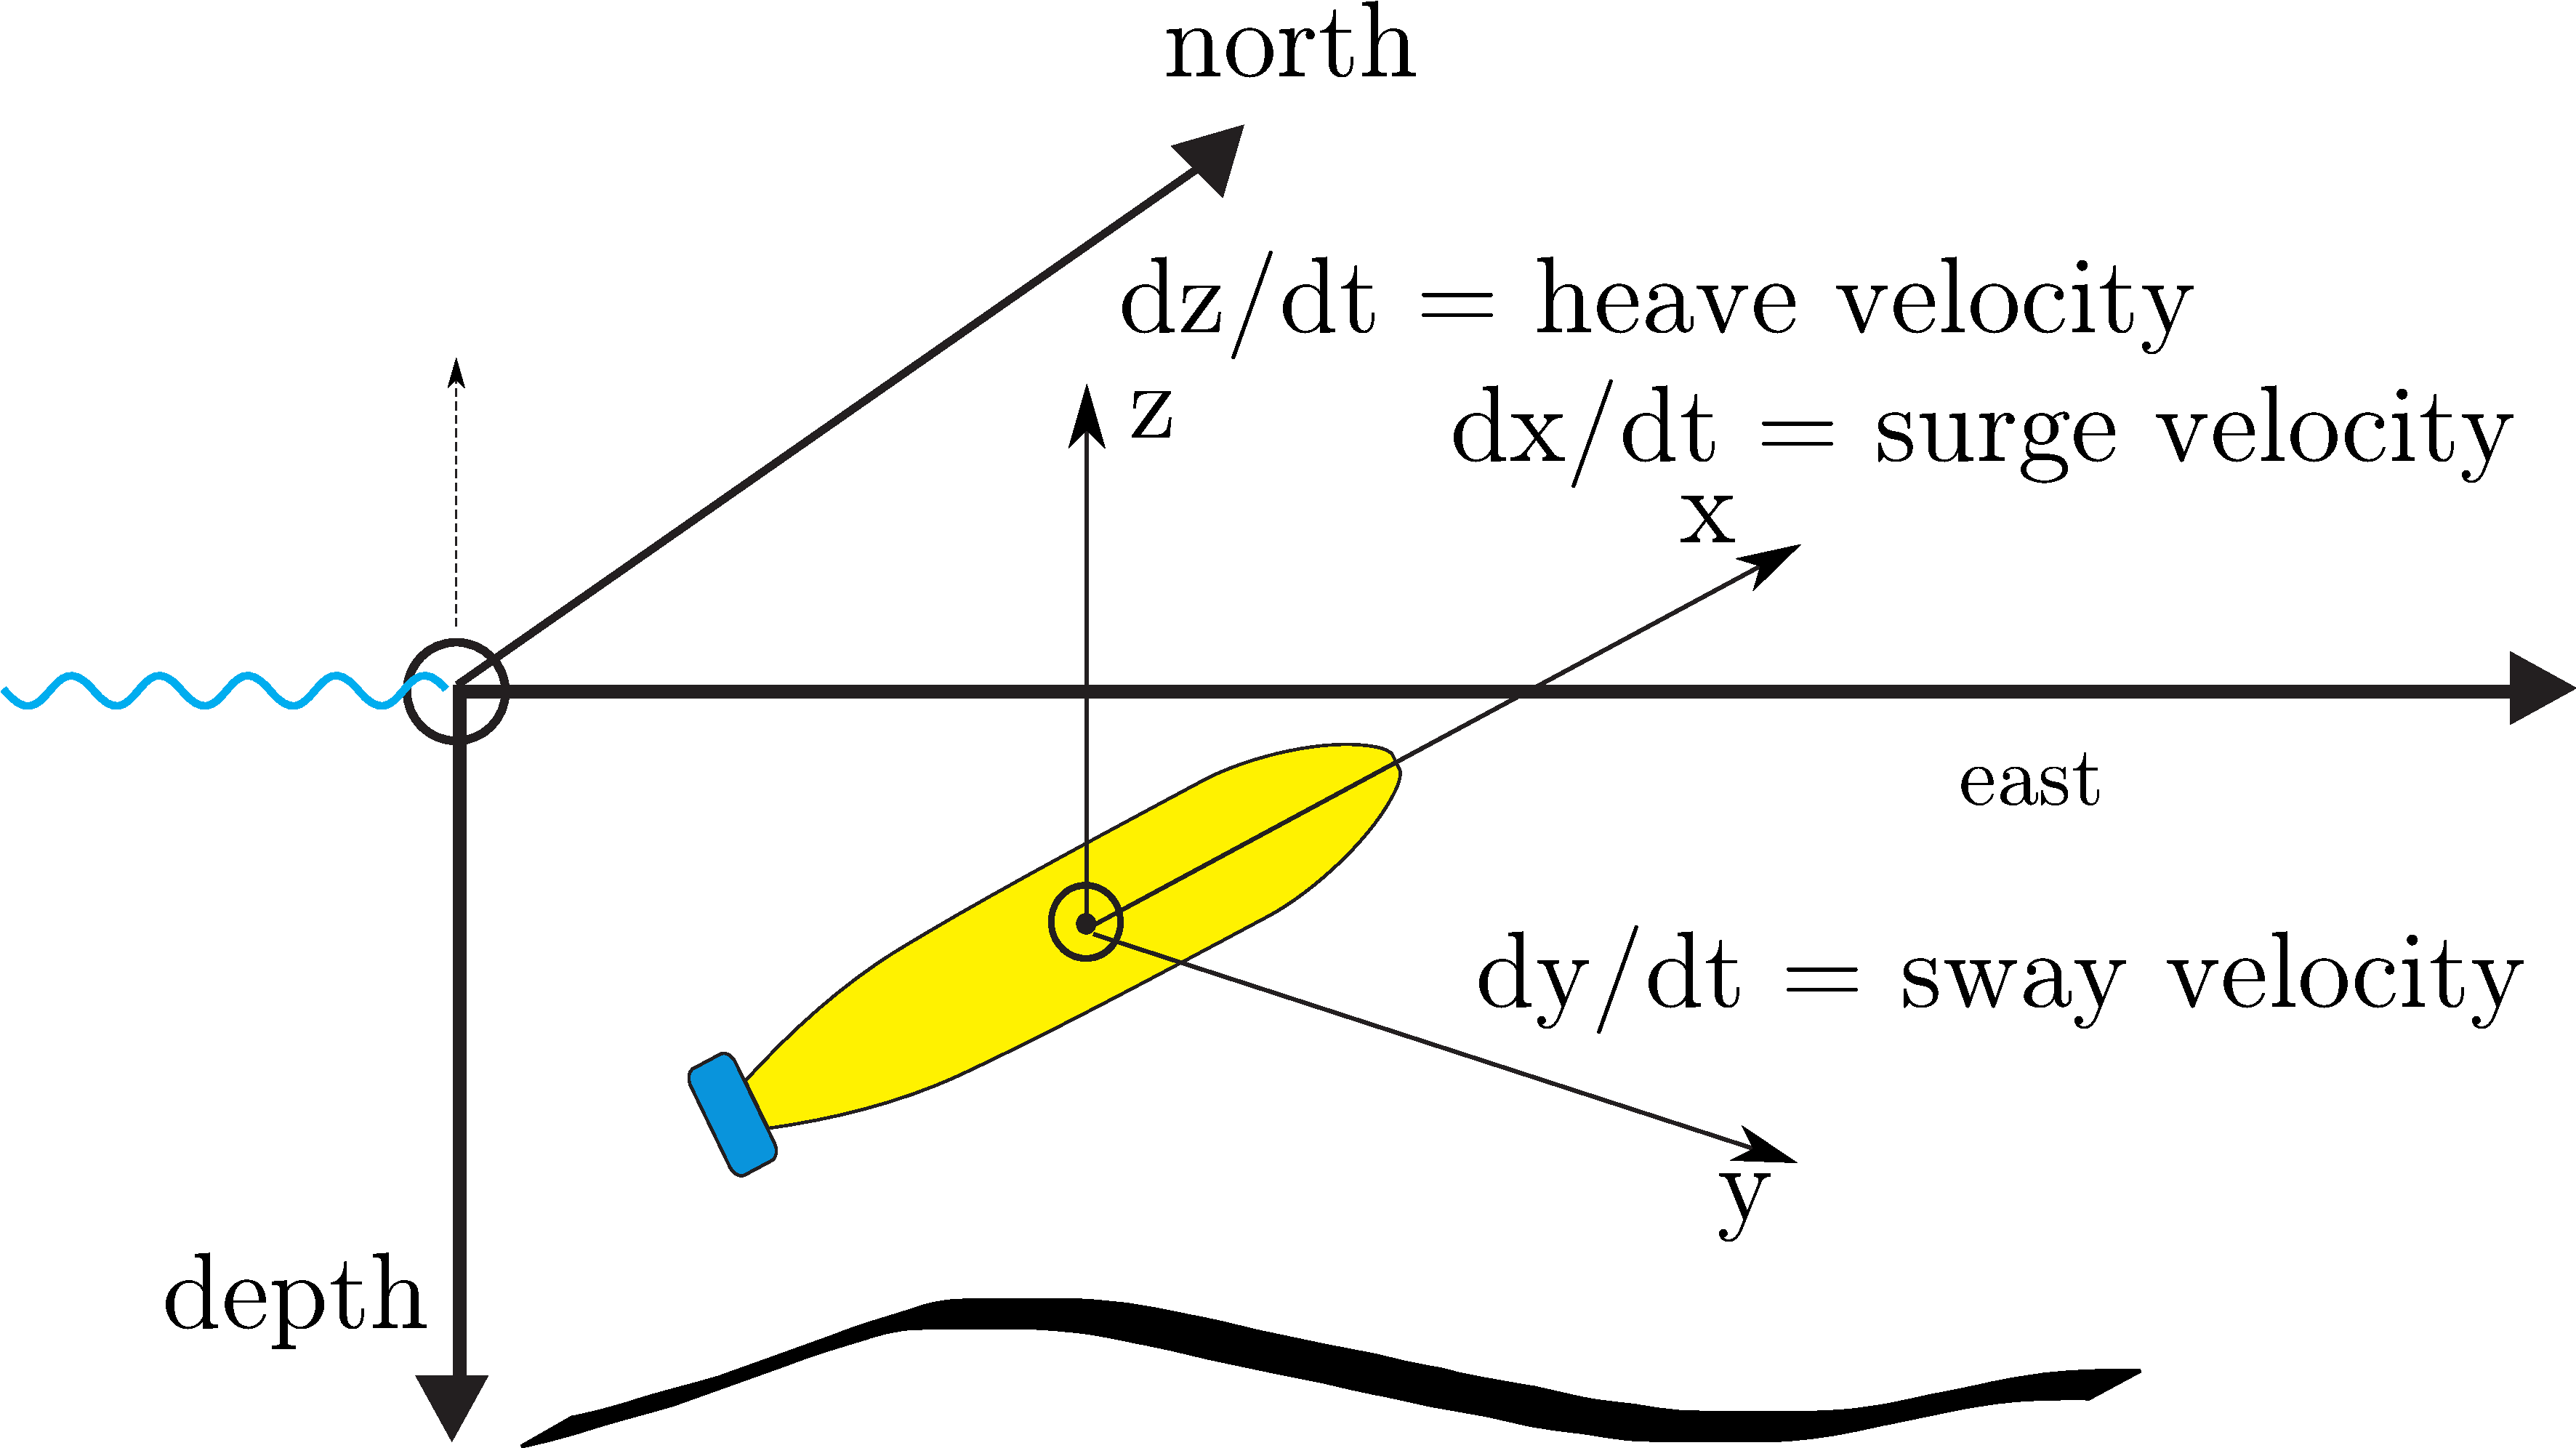
\includegraphics[width=0.8\linewidth]{auv-axes.pdf}}
\caption{AUV state vector values and five degrees of freedom.}
\label{fig:auv-states}
\vspace{-10pt}
\end{figure}
Position, orientation and velocities of a vehicle underwater are stored within the state vector. Proposed solution for localisation uses state-space approach and EKF to estimate the value of the state vector using data from odometry sensors and acoustic positioning system (LBL), if available. Reasons for choosing this method are influenced by the application itself. Localisation is intended to work in unstructured environments, with no clear visibility, relying on kinetic and absolute position measurements.
%Data are merged together using the EKF. 
Mathematical model of the system is the integral part of the EKF. It is used to define the state transition law by applying well known kinematic equations which describe object motion \cite{thrun05}. \textit{Constant velocity} 5DOF kinematic model is used as system model to predict the movements of the submerged body \cite{ribas10}. States are predicted at each time-step using the model $f()$ and previous state $\vect{X}(k-1)$ (equation ~\ref{eq:state-tran}).
\begin{equation}
\vect{X}(k) = f(\vect{X}(k-1), \vect{N}(k-1))
\label{eq:state-tran}
\end{equation}

\textit{Process model} is used to describe the state transition in time. In proposed discrete-time stochastic model, 5DOF include position values and two angle states: yaw and pitch - making altogether five possible values to change in modelling vehicle position (figure ~\ref{fig:auv-positioning}). Since the application uses state-space approach, focus will be on defining a state vector that would incorporate all the relevant values for the dynamic system - kinematic and position variables. In spirit of that, system state vector combines together metric and angular values. At discrete time moment $k$, it values:
$$ \vect{X}(k) = 
\left[ 
\begin{array}{ccccccccccc}
x & y & z & a & u & v & w & \psi & \varphi & \dot{\psi} & \dot{\varphi}
\end{array}
\right] ^{T} $$  
$x$ takes the value of \textit{north} (expressed in meters), $y$ is \textit{east} and $z$ is \textit{depth}. $a$ marks the \textit{altitude} with $u$, $v$ and $w$ standing for linear velocities: \textit{surge}, \textit{sway} and \textit{heave velocity}, respectfully. The rest of the state vector covers angular values (expressed in radians or degrees). $\psi$ and $\varphi$ are used as yaw and pitch, hence describing the vehicle orientation. $\dot{\psi}$ and $\dot{\varphi}$ are angular velocities: yaw rate and pitch rate, respectfully. The state vector incorporates all the relevant information necessary to describe the system under investigation. Angle and velocity for pitch degree of freedom is included in 5DOF system model since it can make a difference in estimating vehicle location in cases of tilted vehicle movement. Model uses previous state and noise to make a prediction on the next state vector value $\vect{X}(k)$  using non-linear function $f()$ and process noise vector $\vect{N}$ (Equation ~\ref{eq:state-tran}) where $\vect{N} = \left[ \begin{array}{ccccc} \dot{u} & \dot{v} & \dot{w} & \ddot{\psi} & \ddot{\varphi} \end{array} \right]^{T}$. Process noise models inaccuracies or unpredictable disturbances in motion model \cite{ristic04}. 
\begin{figure*}%[ht!]
\vspace{-10pt}
%\hrulefill
\begin{equation}
\label{eq:state-tran-matrix}
\begin{bmatrix} x \\ y \\ z \\ a \\ u \\ v \\ w \\ \psi \\ \varphi \\ \dot{\psi} \\ \dot{\varphi} \end{bmatrix}_{(k)} =
\begin{bmatrix} x + (uT+\dot{u}\frac{T^{2}}{2})\cos(\psi)\cos(\varphi) - (vT+\dot{v}\frac{T^{2}}{2})\sin(\psi)\cos(\varphi) \\ 
                y + (uT+\dot{u}\frac{T^{2}}{2})\sin(\psi)\cos(\varphi) + (vT+\dot{v}\frac{T^{2}}{2})\cos(\psi)\cos(\varphi) \\ 
                z + (wT+\dot{w}\frac{T^{2}}{2})\cos(\varphi) \\ 
                a - (wT+\dot{w}\frac{T^{2}}{2})\cos(\varphi) \\ 
                u + \dot{u}T \\ 
                v + \dot{v}T \\ 
                w + \dot{w}T \\ 
                \psi    + \dot{\psi}T    + \ddot{\psi}   \frac{T^{2}}{2} \\ 
                \varphi + \dot{\varphi}T + \ddot{\varphi}\frac{T^{2}}{2} \\ 
                \dot{\psi}    + \ddot{\psi}T \\ 
                \dot{\varphi} + \ddot{\varphi}T
\end{bmatrix}_{(k-1)} 
\end{equation}
%\hrulefill
\vspace{-10pt}
\end{figure*}
To summarize, implementing vehicle localization using EKF demands establishing two models: first one describing the state evolution (\textit{system model}) and the second model that associates noisy measurement with the state (\textit{measurement model}). 

EKF (\S~\ref{sec:ekf}) was chosen for the state estimation as a logic choice being an algorithm that integrates together different sensor measurements, makes a sub-optimal, recursive state estimation and above all, is derived for nonlinear systems \cite{thrun05}. The main feature of EKF is that it linearises the system model and measurement model nonlinear functions. System model is further developed according to formulas ~\ref{eq:der-proc-state}, ~\ref{eq:der-proc-noise}, ~\ref{eq:der-mes-state} and ~\ref{eq:der-mes-noise}.

Knowing plant model and deriving $\vect{F}(k)$, $\vect{W}(k)$ enables EKF algorithm to complete the prediction stage using known formulas. Next step is the correction of the prediction using data obtained from measurement.
\begin{figure}%[htp]
  \begin{center}
    \subfigure[EKF filters after each sensor measurement.]   {\label{fig:asynch}   
    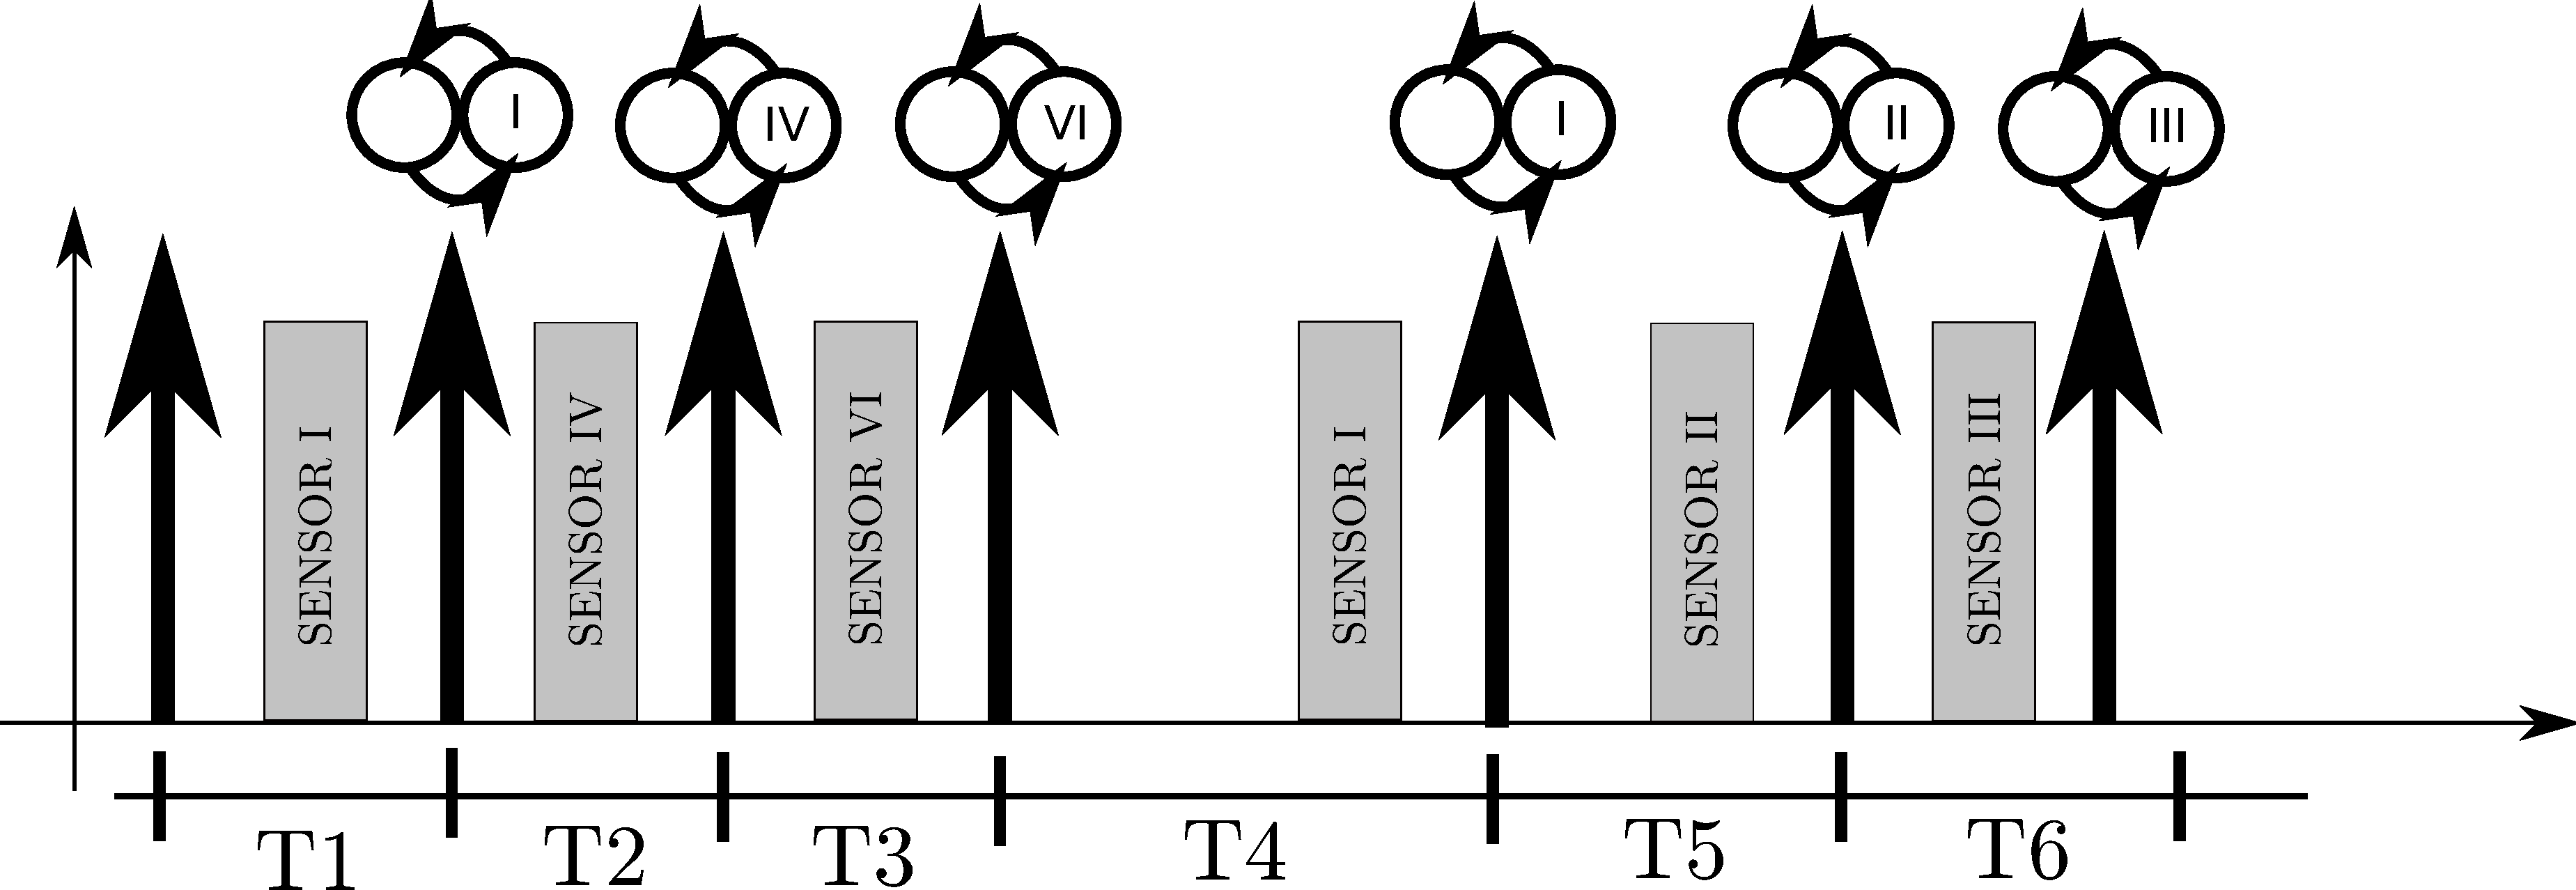
\includegraphics[width=0.4\textwidth]{asynch.pdf}}
    \subfigure[EKF filters periodically.]{\label{fig:synch}
    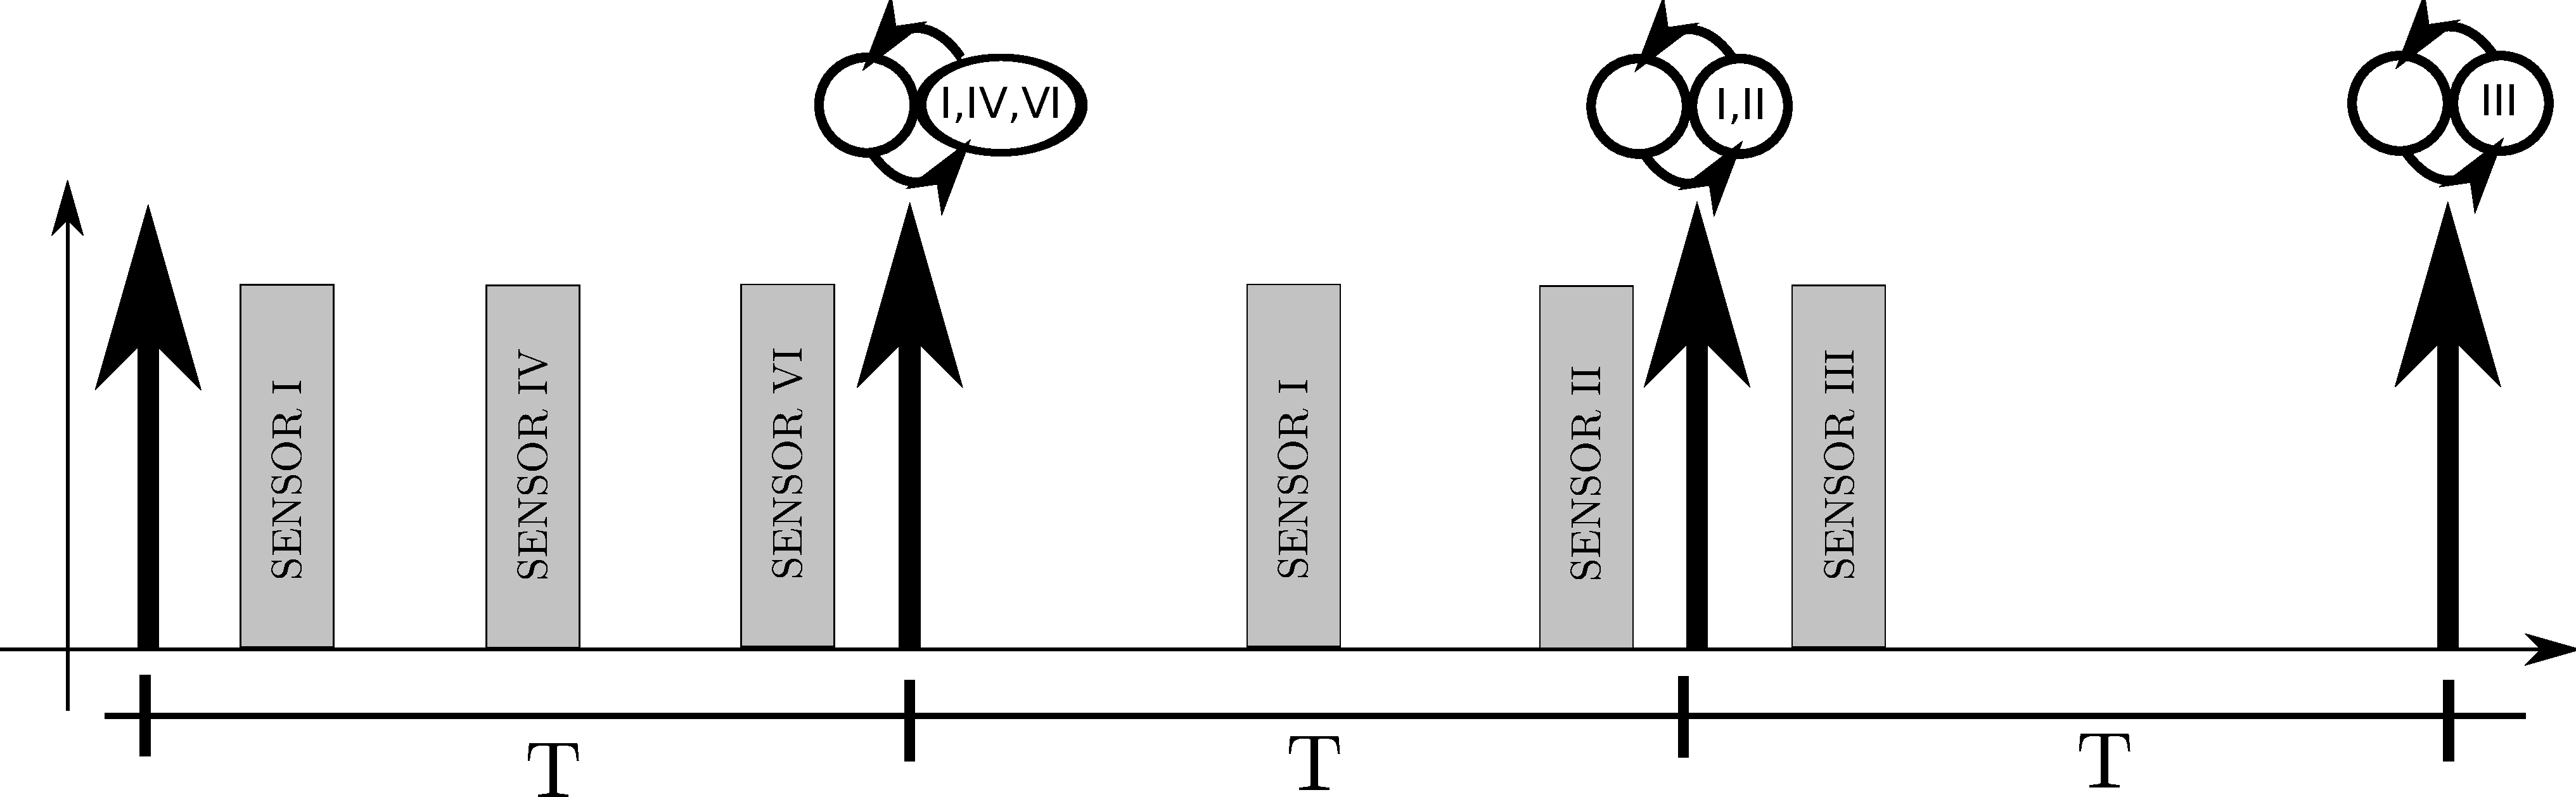
\includegraphics[width=0.4\textwidth]{synch.pdf}}  
  \end{center}
  \caption{Two modes for combining together sensor measurements into observation.}
  \vspace{-10pt}
  \label{fig:ekf-modes}
\end{figure}
\textit{Measurement model} introduces measurement equation which establishes the connection between the measurements and the target state (equation ~\ref{eq:mes-model}) where $Z(k)$ represents the measurement at time $k$, $X(k)$ represents state vector and $M(k)$ represents noise. Purpose of the measurement is to be able to update, correct the state $X(k)$ using measurements $Z(k)$. $h()$ is generally a non-linear function. EKF linearises the measurement model.
\begin{equation}
\vect{Z}(k) = h(\vect{X}(k), \vect{M}(k)) = \vect{H} \vect{X}(k \mid k-1)  + \vect{M}(k)
\label{eq:mes-model}
\end{equation}
%$h()$ can be expressed with matrix containing ``ones'' at particular positions since
For this particular application and available sensor configuration, state vector elements are measured directly, hence the measurement relation becomes equality. There is no need for partial derivation (Equation ~\ref{eq:mes-model}). Measurement noise is submitted in form of an additive Gaussian zero-mean noise assigned to each measured value. Measurement (observation) noise is characterised with zero mean $(E \lbrace \vect{M}(k) \rbrace = \vect{0})$ and standard deviation $(E \lbrace \vect{M}(k) \vect{M}^{T}(k) \rbrace)$ given as diagonal covariance matrix with diagonal elements set to constant filter parameter $\sigma^{2}$ for each of the measured values (Figure ~\ref{eq:concatenate-mes}). It expresses how much we trust in the measurement, how uncertain or varying measurement of each of the state values is. 

One of the features of the process is that measurements are not available all the time. The reason is the nature of the process of estimating the location itself. Simply - messages from sensors arrive at different moments and it happens that some of the sensors could not be available due to different causes (no ``dvl lock'', for instance). The idea is to take all the available information periodically and integrate it together in measurement model, as a filter observation (Figure ~\ref{fig:synch}). Alternatively, each message can be filtered upon its arrival (Figure ~\ref{fig:asynch}). In case observation is empty, filter does the prediction only. Idea for the solution has been introduced in \cite{ribas10}. Some other implementations of EKF for underwater navigation have reported the usage of similar strategy for merging the measurements together \cite{drolet00, blain03}. This way, measurement model adopts to the set of the values observed.

Integrating together several different sensor-specific measurements into one observation would imply concatenating together several measurement matrices $(\vect{Z}, \vect{H})$ and measurement noise matrices $(\vect{R})$, as shown in ~\ref{eq:concatenate-mes} for the sample case of two sensor device measurements included in one observation. EKF maintains its own timer for the observations (value T from the model). As an example, depth sensor measures depth $(z)$ and heave velocity $(w)$, thus $$\vect{Z}_{depth} =\left[\begin{array}{cc} z & w \end{array} \right] ^{T}$$, $$\vect{H}_{depth} =\left[\begin{array}{ccccccccccc} 0 & 0 & 1 & 0 & 0 & 0 & 0 & 0 & 0 & 0 & 0 \\ 0 & 0 & 0 & 0 & 0 & 0 & 1 & 0 & 0 & 0 & 0 \end{array} \right]$$ and $$\vect{R}_{depth} =\left[\begin{array}{cc} \sigma_{depth}^{2} & 0 \\ 0 & \sigma_{w}^{2} \end{array} \right] $$. Where $\sigma$ marks the standard deviation expressing how much we trust in  measurement. It is given as EKF parameter. Similar pattern values for the other sensors depending on values that they measure.
\begin{figure*}
\begin{equation}
\label{eq:concatenate-mes} 
\vect{Z}(k) = \left[ \begin{array}{c} \vect{Z}_{sensor I} \\ \vect{Z}_{sensor II}  \end{array} \right],
\vect{H}(k) = \left[ \begin{array}{c} \vect{H}_{sensor I} \\ \vect{H}_{sensor II}  \end{array} \right], 
\vect{R}(k) = \left[ \begin{array}{ccc} \vect{R}_{sensor I} & 0 \\ 0 & \vect{R}_{sensor II} \end{array} \right]
\end{equation}
\vspace{-10pt}
\end{figure*}
%\\ \vect{Z}_{sensor III} \\ \vect{H}_{sensor III}  & 0  & 0    \\ 0 & 0 & \vect{R}_{sensor III}
Having more than one measurement involved in estimation of the global state is a good characteristic. The estimate which uses more diverse data gives better estimate since it is possible to combine together more that one sort of observation. Another advantage follows the fact that the whole set of state variables is updated each time, resulting in more correlation between variables. Hence those that are missing for some reason can be compensated this way. Results of simulations using authentic data and the  real missions are given in Section \S~\ref{sec:results}. Odometry integrates velocity and acceleration data collected from devices such as gyroscope or accelerometers. Integration of noisy data over time or usage of ``relative measurements'' (those calculated from absolute measurements) results in drift or bias of the final estimate. In order to recover from that, algorithms perform the correction. Correction takes an absolute measurement which should be less precise, possibly noisy, but not prone to drifting. %An example which illustrates the phenomenon could be a man that walks with the eyes closed trying to keep the track of his position by measuring the steps and predicting where he could possibly be judging on number of steps and their size. Steps have the role of ``relative measurement'' - one quantity is used to estimate the other one that's correlated with it. Naturally, a man will keep making errors in his position estimate. Moreover, these errors will accumulate over time producing drift. Correction would require the man to open his eyes and observe the current position (absolute measurement), compare it with the position predicted by counting steps and neutralise the drift before carrying on with the eyes closed. 